
\begin{frame}[fragile]
\frametitle{Algoritmos y programaci\'on (1)}
\begin{columns}
\column{0.55\linewidth}

\begin{block}{Algoritmo}
Conjunto finito de instrucciones para resolver una tarea espec\'ifica \pause
\end{block}

\begin{itemize}
\item Las instrucciones deben ser claras (no ambig\"uas) \pause
\item El orden debe estar definido, de tal forma que si no efectuan los pasos en el orden, no se logra el objetivo \pause
\end{itemize}

\column{0.35\linewidth}
 
\begin{center}
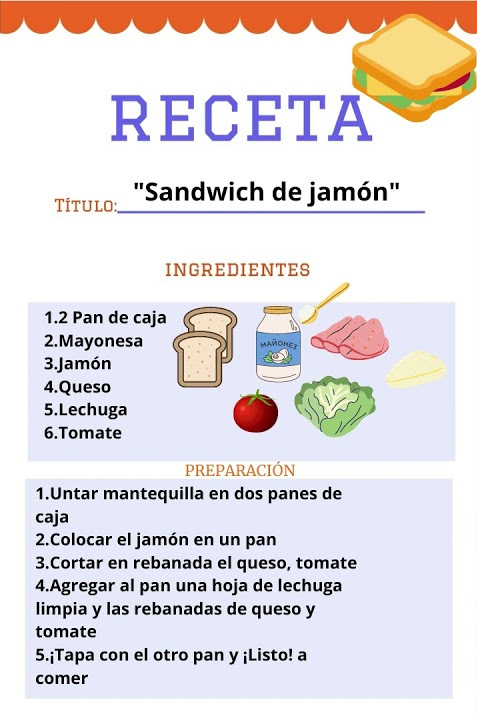
\includegraphics[width=0.85\textwidth]{Figs/receta_sandwidch.jpg}
\end{center} 
\end{columns}

\end{frame}

\begin{frame}[fragile]
\frametitle{Algoritmos y programaci\'on (2)}

\begin{block}{Variable}
Un espacio reservado para almacenar un dato \pause
\end{block}

\begin{center}
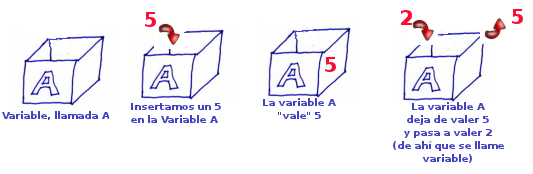
\includegraphics[width=0.45\textwidth]{Figs/que_es_una_variable.png} \pause
\end{center} 

\begin{block}{Arreglo}
Una coleccion ordenada de variables del mismo tipo, que puede ser accesada por un indice\pause
\end{block}

\begin{center}
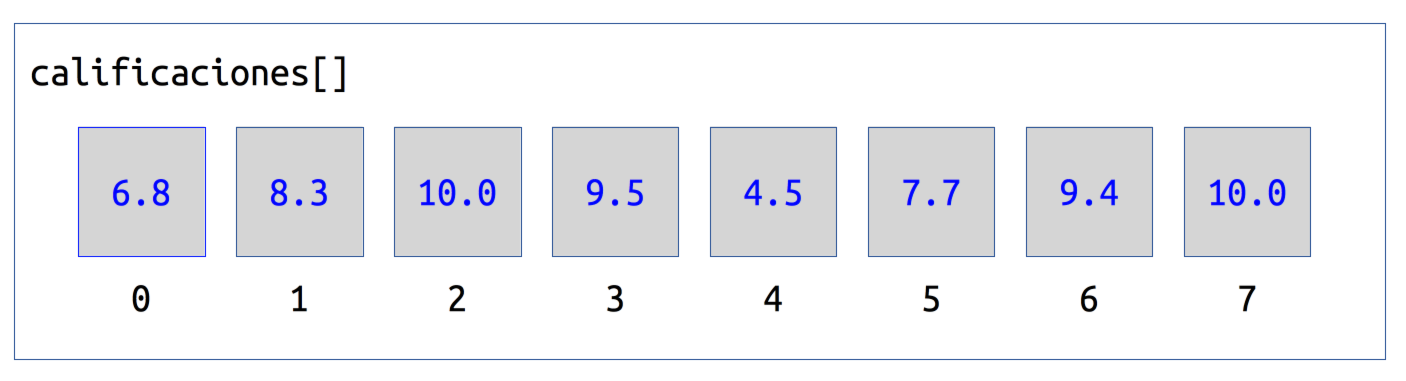
\includegraphics[width=0.55\textwidth]{Figs/arreglos1.png}
\end{center} 


\end{frame}


\begin{frame}[fragile]
\frametitle{Algoritmos y programaci\'on (3)}

\begin{block}{Obtener la mayor estatura y el lugar de la fila del niño(a) de mayor estatura}
\begin{center}
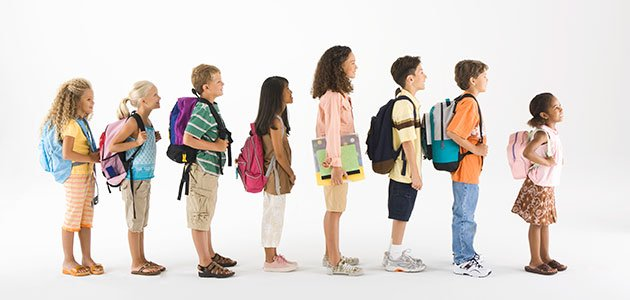
\includegraphics[width=0.45\textwidth]{Figs/fila_ninos.jpg} \pause
\end{center}  
\end{block}

\begin{itemize}
\item Medir o preguntar la estatura de los niños (En orden o en desorden?) \pause
\item Analizar las estaturas para obtener la mayor. \pause
\item Respaldar (escribir en alguna parte) la altura (o el lugar en la lista) del niño mas alto.  \pause
\end{itemize}

\end{frame}





\begin{frame}[fragile]
\frametitle{Algoritmos y programaci\'on (4)}
\begin{columns}
\column{0.45\linewidth}
\begin{block}{Obtenci\'on de estaturas}
\begin{minted}[linenos,fontsize=\tiny]{c}
numero_ninos = 8;    
int Estaturas[numero_ninos]; //Estatura en Centimetros
indice = 0;
while (indice<numero_ninos) 
{   
    EstaturaActual = preguntarEstatura(indice)
    Estaturas[indice]=EstaturaActual
    indice=indice+1
}      
\end{minted} 
\pause
\end{block}

\begin{block}{Estructura de Control Repetitiva (while)}
Permite ejecutar un grupo de instrucciones por X cantidad de veces \pause
\end{block}
\column{0.45\linewidth}
\begin{block}{An\'alisis de las estaturas}
\begin{minted}[linenos,fontsize=\tiny]{c}
numero_ninos = 8;
indice = 0;
while (indice<numero_ninos) 
{   
    if (indice == 0){        
        mas_alto = indice  
        estatura_mas_alto=Estaturas[indice]     
    } 
    else 
    {
        if (Estaturas[indice]>mas_alto) {
            mas_alto = indice
            estatura_mas_alto=Estaturas[indice]     
        }
    }
    indice=indice+1
}      
\end{minted} 
\pause
\end{block}

\begin{block}{Estructura de Control Selectiva (IF)}
Permite ejecutar instrucciones basados en una condicion \pause
\end{block}

\end{columns}




\end{frame}


\begin{frame}
\frametitle{Algoritmos y programaci\'on (5)}
\begin{columns}
\column{0.45\linewidth}

\begin{block}{Computadora}
Es una m\'aquina (electr\'onica) programable* que recibe y procesa datos para convertirlos en informaci\'on \'util. Contiene perif\'ericos de entrada (para introducir datos) y salida (para mostrar resultados) \pause
\end{block}


\begin{block}{Programa de Computadora}
Un conjunto de instrucciones escritas en un lenguaje de programaci\'on, que una computadora interpreta en una secuencia l\'ogica para llevar a cabo una tarea en particular \pause
\end{block}


\column{0.45\linewidth}


\begin{block}{Lenguaje de Programaci\'on}
Un lenguaje que permite a un programador codificar instrucciones que ser\'an ejecutadas por una computadora. \pause
\end{block}

\end{columns}
\end{frame}


\begin{frame}[fragile]
\frametitle{Algoritmos y programaci\'on (6)}

\begin{columns}
\column{0.58\linewidth}

\begin{block}{Programa en Python para Leer estaturas}
\inputminted[linenos,fontsize=\tiny]{python}{00_ConceptoAlgoritmo_Ninos/Estaturas.py}
\end{block}


\column{0.42\linewidth}
\begin{center}

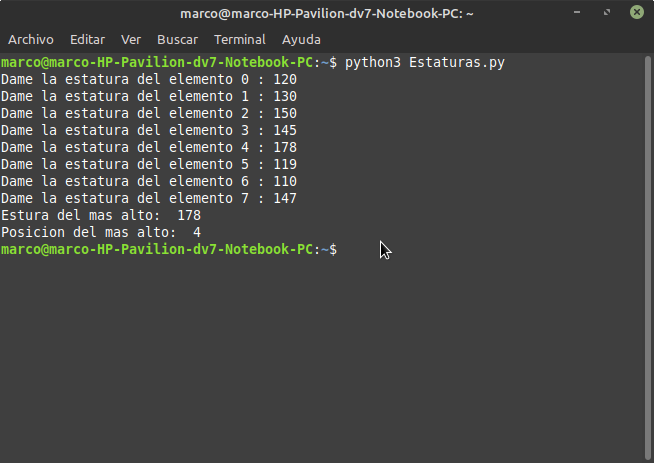
\includegraphics[width=0.95\textwidth]{00_ConceptoAlgoritmo_Ninos/Ejecucion_Estaturas.png} \pause
\end{center} 

\end{columns}
\end{frame}



\begin{frame}
\frametitle{Sistema Operativo}  
\begin{columns}
%\column{0.32\linewidth}
\column{0.65\linewidth}
\begin{block}{}
Un Sistema Operativo (SO) es un programa (software) que al arrancar la computadora** se encarga de gestionar todos los recursos del sistema informático permitiendo así la comunicación entre el usuario y la computadora. 
\end{block}
\begin{center}
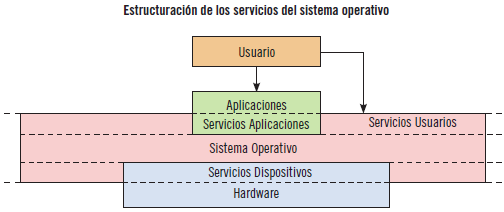
\includegraphics[width=0.95\linewidth]{00_IntroProgramacionYMoviles/SistemaOperativo1.png} 
\end{center}
\tiny{\url{https://reader.digitalbooks.pro/content/preview/books/38230/book/OEBPS/Text/c1.html}}

\column{0.32\linewidth}
\begin{center}
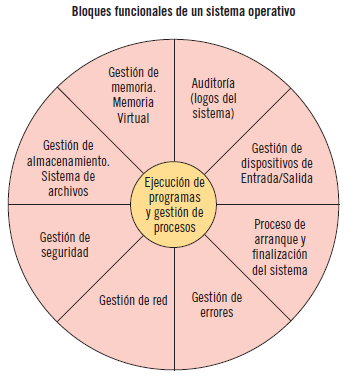
\includegraphics[width=0.95\linewidth]{00_IntroProgramacionYMoviles/SistemaOperativo2.png} 
\end{center}
\end{columns}

\end{frame}


\begin{frame}
\frametitle{Sistemas Operativos para PCs}  

\begin{columns}
\column{0.32\linewidth}
\begin{center}

\includegraphics[width=0.95\linewidth]{00_IntroProgramacionYMoviles/Windows11.png} 
\end{center}

\column{0.32\linewidth}
\begin{center}
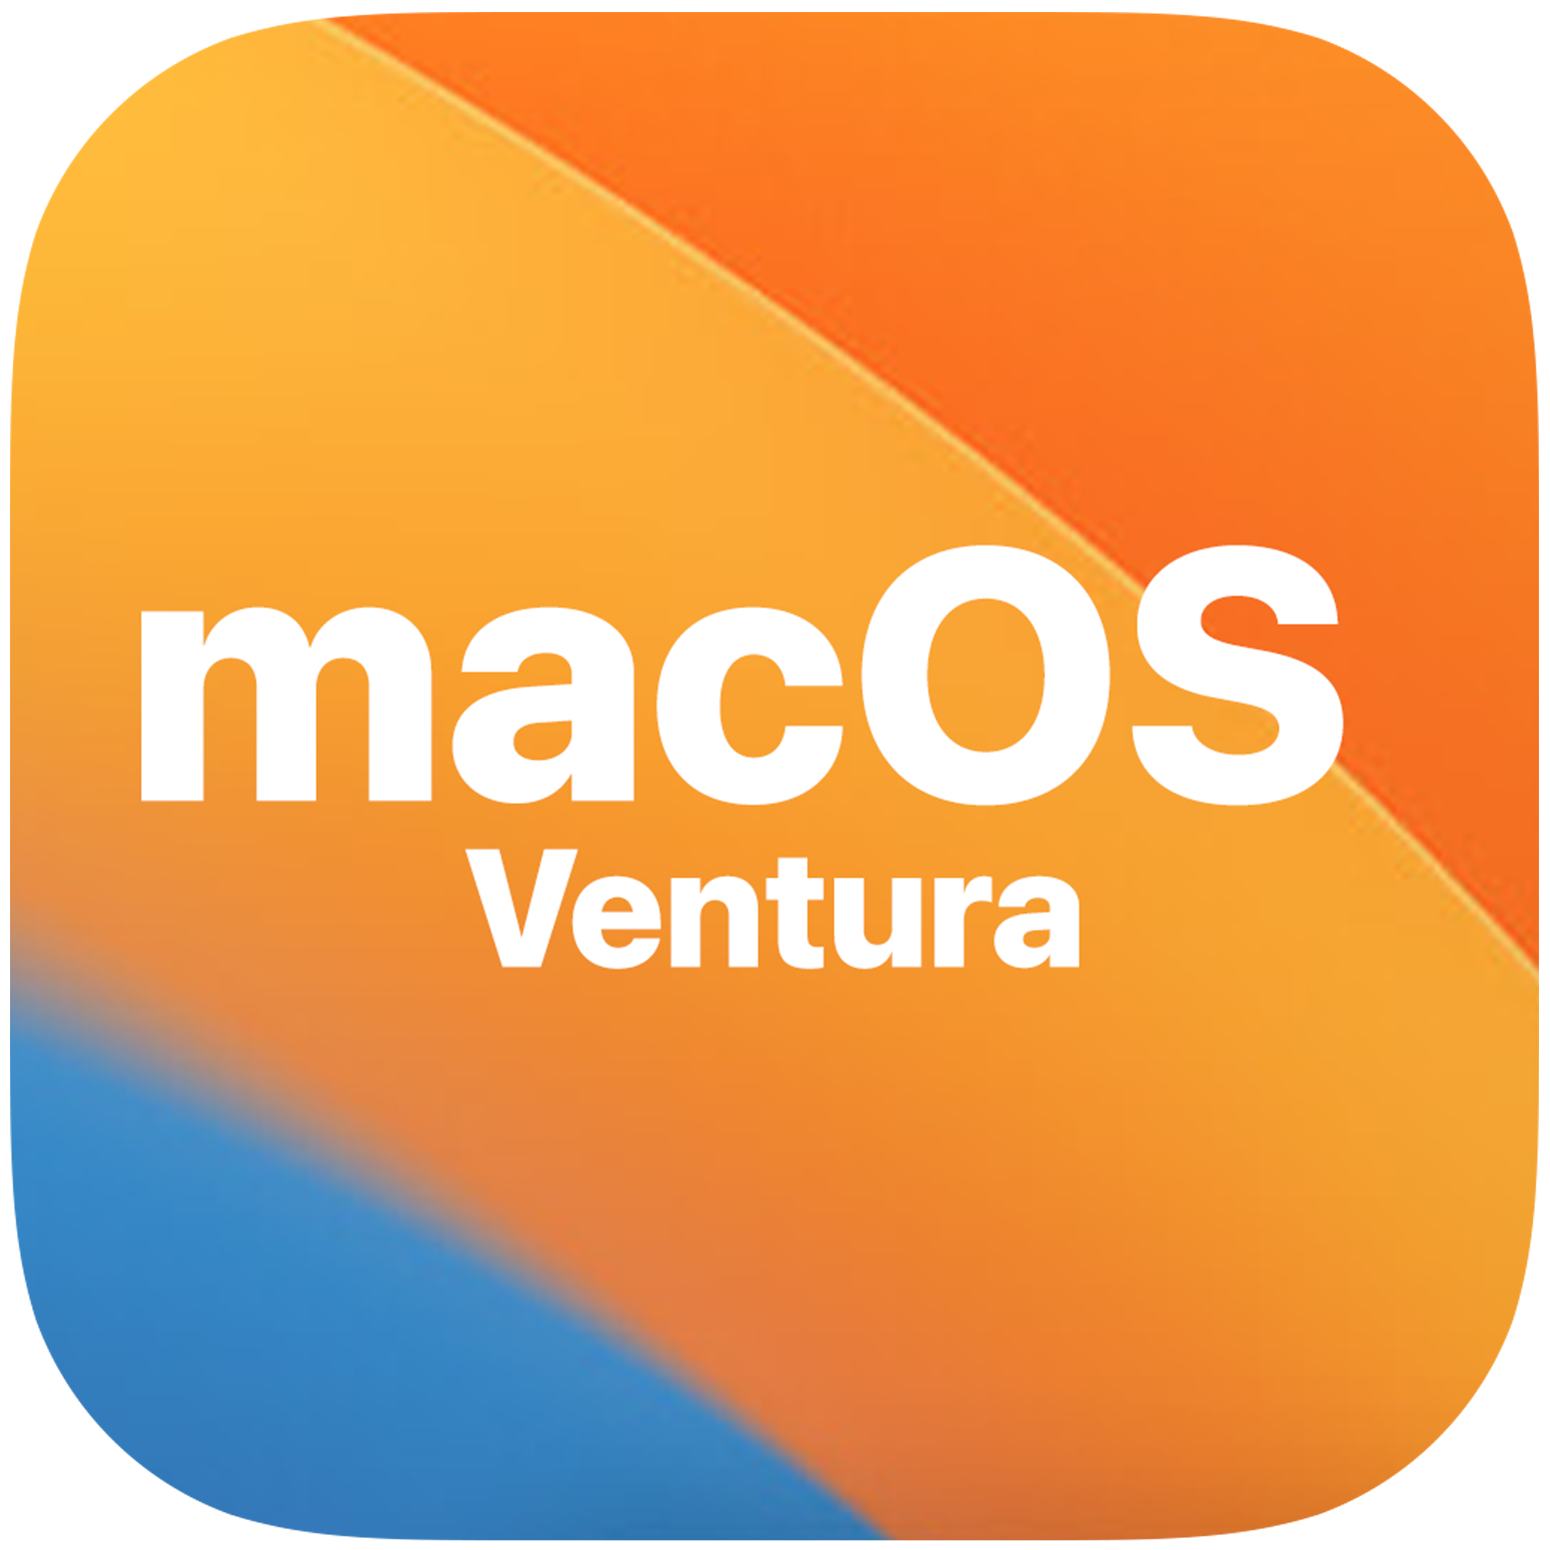
\includegraphics[width=0.95\linewidth]{00_IntroProgramacionYMoviles/MacOS.png} 
\end{center}

\column{0.32\linewidth}
\begin{center}

\includegraphics[width=0.95\linewidth]{00_IntroProgramacionYMoviles/Linux.png} 
\end{center}
\end{columns}

\end{frame}





\begin{frame}
\frametitle{Telefono Celular No-inteligente vs Telefono Celular Inteligente}  

\begin{columns}
\column{0.46\linewidth}
\begin{block}{Tel\'efono No-inteligente}
\begin{itemize}
\item Su funcionalidad principal era la comunicaci\'on (llamadas o mensajes) a trav\'es de la red celular (GSM)
\end{itemize}
\end{block}
\begin{block}{Tel\'efono inteligente}
\begin{itemize}
\item Interfaz de entrada: Pantalla Touch (a color, de alta definici\'on) 
\item Conexi\'on a Internet: WiFi, GSM (4G o 5G)
\item Comunicaci\'on con otros dispositivos: Bluetooth, NFC
\item C\'amaras (Frontal y Posterior)
\end{itemize}
\end{block}

\column{0.18\linewidth}
\begin{center}
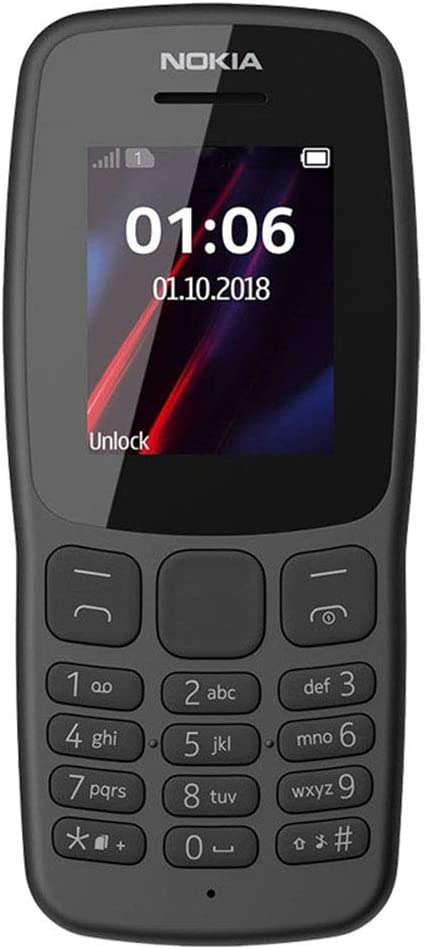
\includegraphics[width=0.95\linewidth]{00_IntroProgramacionYMoviles/FeaturePhone_Nokia.png} 
\end{center}
\column{0.28\linewidth}
\begin{center}
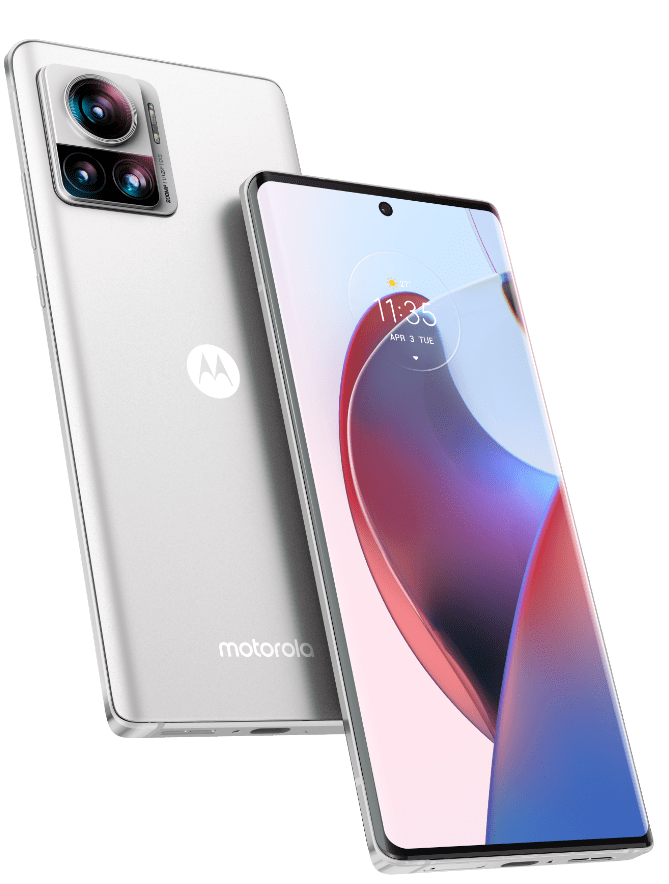
\includegraphics[width=0.95\linewidth]{00_IntroProgramacionYMoviles/Smartphone_Motorola.png} 
\end{center}
\end{columns}
\end{frame}

\begin{frame}
\frametitle{Sistemas Operativos para Telefonos Inteligentes} 
\begin{columns}
\column{0.32\linewidth}
\begin{center}

\includegraphics[width=0.95\linewidth]{00_IntroProgramacionYMoviles/Android.png} 
\end{center}

\column{0.32\linewidth}
\begin{center}
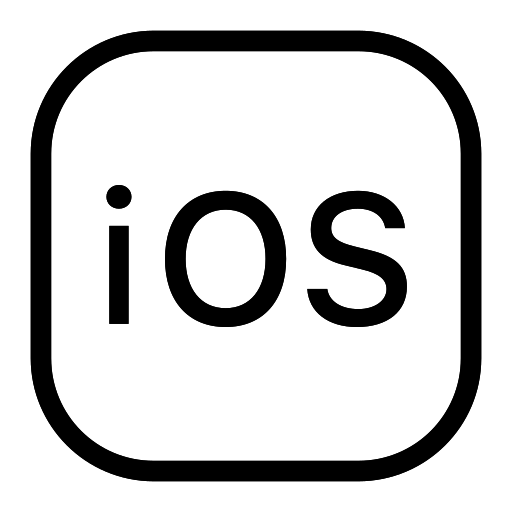
\includegraphics[width=0.95\linewidth]{00_IntroProgramacionYMoviles/iOs.png} 
\end{center}

\column{0.32\linewidth}
\begin{center}
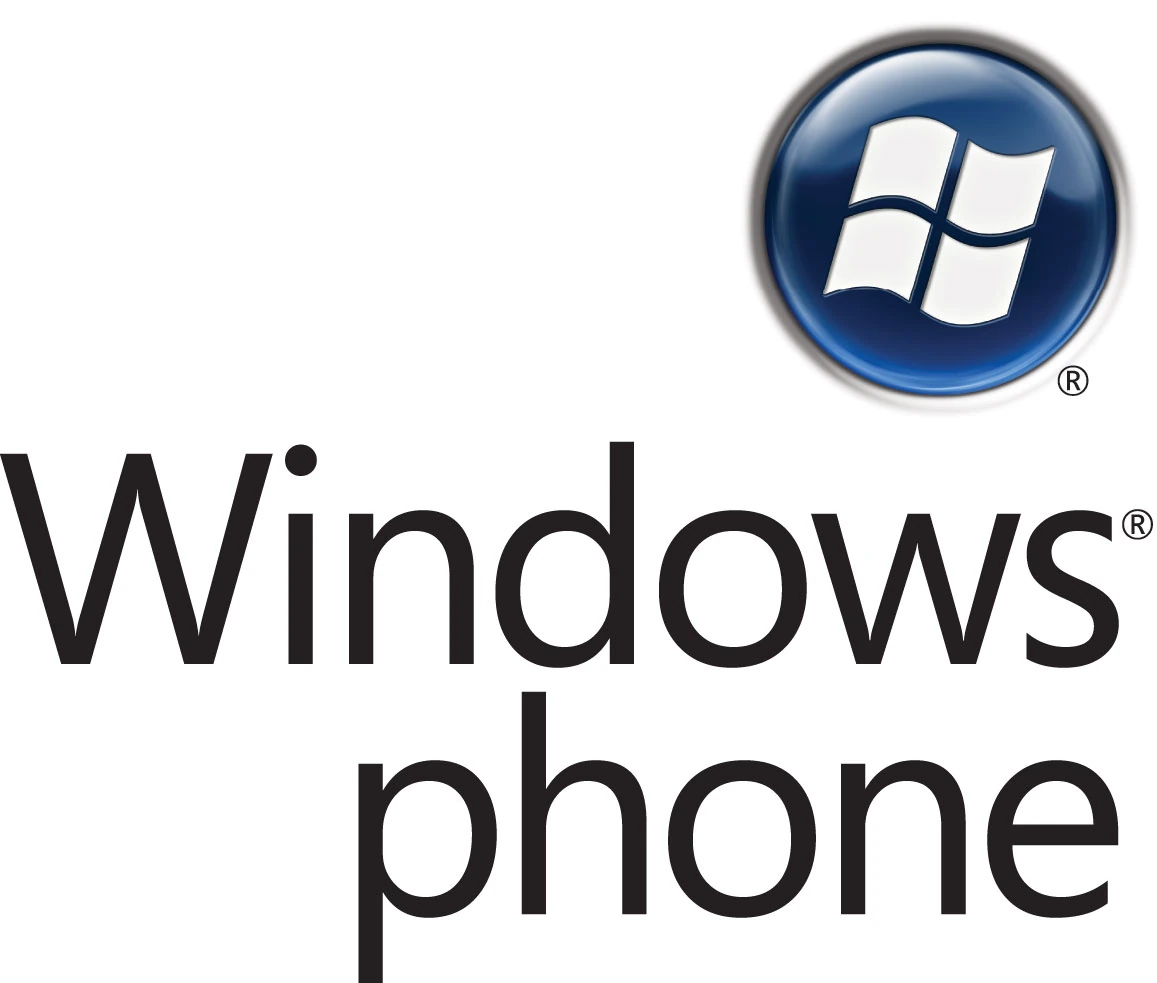
\includegraphics[width=0.95\linewidth]{00_IntroProgramacionYMoviles/WindowsPhone.png} 
\end{center}
\end{columns}
 
\end{frame}


\begin{frame}
\frametitle{Android} 
\begin{columns}
\column{0.64\linewidth}
\begin{itemize}
\item Android es un sistema operativo móvil basado en Linux 
\item Principalmente orientado a dispositivos de pantalla t\'actil (Smartphone, tablets, smartwatches, etc)
\item Fue desarrollado por Android Inc (Adquirida por Google en 2005)
\item Vinculado con un grupo de empresas (HTC, Sony, Motorola, Samsung, LG, Lenovo, entre otras) para la creaci\'on de un SO com\'un para sus dispositivos
\item A la fecha (Q1 2023), los tel\'efonos con SO Android concentran mas del 70\% del mercado global. 
\end{itemize}
\column{0.32\linewidth}
\begin{center}
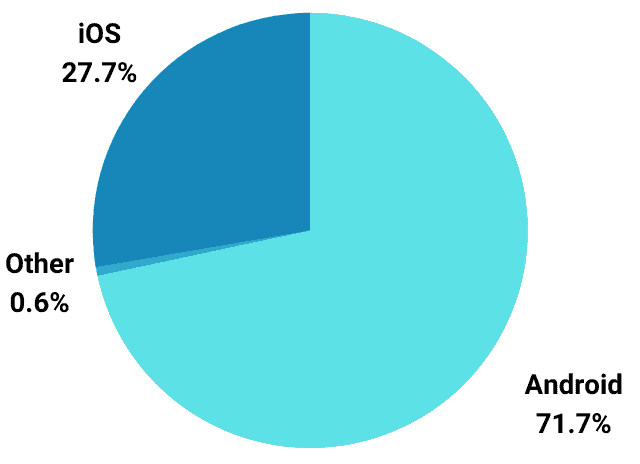
\includegraphics[width=0.95\linewidth]{00_IntroProgramacionYMoviles/AndroidVSIOs_WorldWide.png} 
\end{center}
\end{columns}
 
\end{frame}





\begin{frame}
\frametitle{Aplicaciones Móviles}  
\begin{columns}
\column{0.4\linewidth}
\begin{itemize}
\item Ejecutadas en el tel\'efono
\item La entrada de datos es mediante un teclado ``virtual''
\item El apuntador del raton es la pantalla 
\item Incluyen una interfaz de usuario gr\'afica (GUI) 
\item Es posible descargar miles de \'estas en nuestros dispositivos
\end{itemize}
\column{0.30\linewidth}
\begin{center}
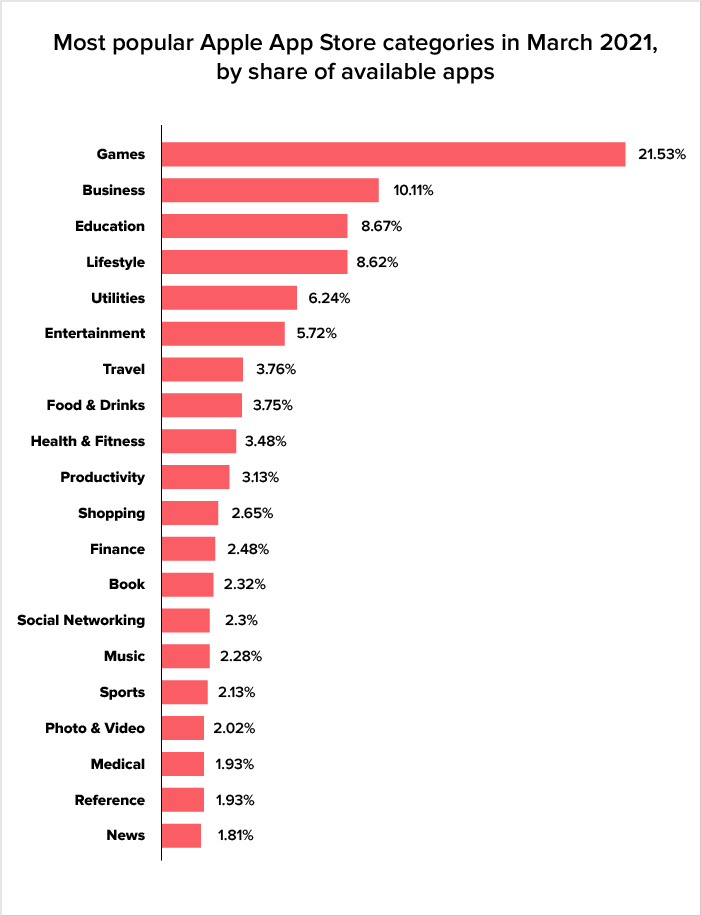
\includegraphics[width=0.95\linewidth]{00_IntroProgramacionYMoviles/TiposAplicaciones.png} 
\end{center}
\column{0.30\linewidth}
\begin{center}
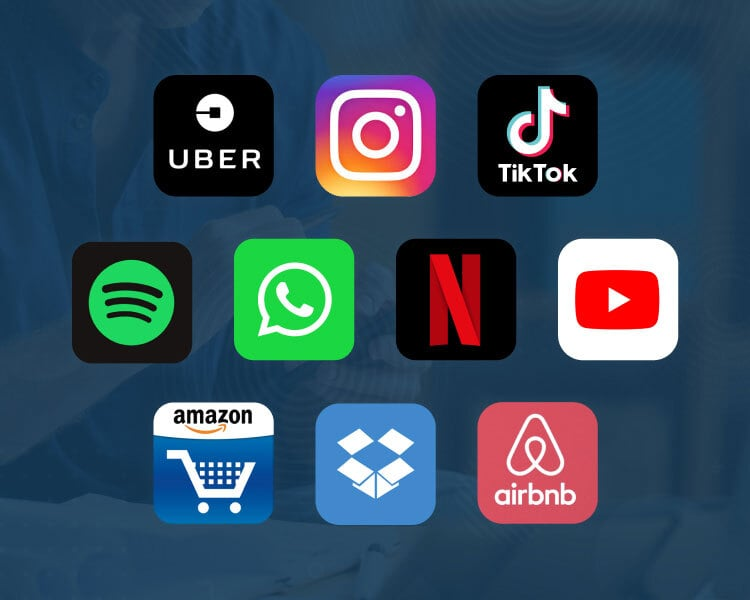
\includegraphics[width=0.95\linewidth]{00_IntroProgramacionYMoviles/most-popular-apps.jpg} 
\tiny{\url{https://www.netsolutions.com/insights/top-10-most-popular-apps-2018/}}  
\end{center}
\end{columns}
\end{frame}



